% Created 2021-02-24 mer. 09:12
% Intended LaTeX compiler: pdflatex
\documentclass[11pt]{article}
\usepackage[utf8]{inputenc}
\usepackage[T1]{fontenc}
\usepackage{graphicx}
\usepackage{grffile}
\usepackage{longtable}
\usepackage{wrapfig}
\usepackage{rotating}
\usepackage[normalem]{ulem}
\usepackage{amsmath}
\usepackage{textcomp}
\usepackage{amssymb}
\usepackage{capt-of}
\usepackage{hyperref}
\usepackage{color}
\usepackage[english]{babel}
\usepackage{a4wide}
\usepackage{mathpazo}
\usepackage{amsmath}
\usepackage{titlesec}
\titlelabel{\thetitle.\quad}
\usepackage[usenames,dvipsnames]{xcolor} % For colors with friendly names
\usepackage{minted}
\usepackage{mdframed}                    % Companion of minted for code blocks
\usepackage{fancyvrb}                    % For verbatim R outputs
\usemintedstyle{friendly} % set style if needed, see https://frama.link/jfRr8Lpj
\mdfdefinestyle{mystyle}{linecolor=gray!30,backgroundcolor=gray!30}
\BeforeBeginEnvironment{minted}{%
\begin{mdframed}[style=mystyle]}
\AfterEndEnvironment{minted}{%
\end{mdframed}}
%% Formatting of verbatim outputs (i.e., outputs of R results):
\DefineVerbatimEnvironment{verbatim}{Verbatim}{%
fontsize = \small,
frame = leftline,
formatcom = {\color{gray!97}}
}
\usepackage{float}
\usepackage{url}
%% Decalre new unicode characters for displaying trees:
\DeclareUnicodeCharacter{2514}{\mbox{\kern.23em \vrule height2.2exdepth-1.8ptwidth.4pt\vrule height2.2ptdepth-1.8ptwidth.23em}}
\DeclareUnicodeCharacter{2500}{\mbox{\vrule height2.2ptdepth-1.8ptwidth.5em}}
\author{Frédéric Santos\thanks{frederic.santos@u-bordeaux.fr}}
\date{\today}
\title{Customizing and extending Emacs Speaks Statistics\\\medskip
\large Part of the ESS-Intro series}
\hypersetup{
 pdfauthor={Frédéric Santos},
 pdftitle={Customizing and extending Emacs Speaks Statistics},
 pdfkeywords={},
 pdfsubject={},
 pdfcreator={Emacs 27.1 (Org mode 9.4.4)}, 
 pdflang={English}}
\begin{document}

\maketitle
\tableofcontents


\section{Introductory words}
\label{sec:org5616365}
\subsection{A short tutorial for customizing ESS}
\label{sec:org1335ccb}
This document is a part of the ESS-Intro tutorial series. A full list of tutorials is available online at \url{https://github.com/ess-intro}.

If you are are totally new to Emacs, you should probably begin with the tutorial ``\href{https://github.com/ess-intro/presentation-first-steps}{First steps with Emacs}'' by Dirk Eddelbuettel.

\subsubsection{Target audience}
\label{sec:orgd74fcb2}
This tutorial is for R-users beginning to use Emacs Speaks Statistics (ESS). We only assume that you have mild familiarity with Emacs, and that you know how to customize Emacs by filling your \texttt{.emacs} or \texttt{init.el} file.

\subsubsection{Goals}
\label{sec:org4ad6e33}
\begin{itemize}
\item Helping newcomers and beginners to have a more friendly and efficient setup
\item Helping users migrating from other IDEs to keep behaviours and habits they are used to
\item Showcasing some other Emacs packages that play well with ESS and may improve your coding experience
\end{itemize}

\subsubsection{Video tutorial}
\label{sec:org4c876f6}
This document is a written companion for the video tutorial available at:

\begin{center}
\url{http://toto}
\end{center}


\subsubsection{An opinionated tutorial?}
\label{sec:orgfe0e2c5}
Some parts of this tutorial (e.g., replacing \texttt{Flymake} by \texttt{Flycheck} for syntax checking, or using \texttt{company} instead of other solutions for auto-completion) might be seen as quite opinionated. However, when several options or approaches were available for a given task, the most widespread and efficient (I hope!) was presented.

If you prefer other approaches, or simply want to give a try to some other ones, the ESS manual remains the canonical and exhaustive documentation: \url{http://ess.r-project.org/Manual/ess.html}

Feedbacks, fixes and contributions are welcome, and can be addressed \href{https://github.com/ess-intro/presentation-ess-customization/issues}{through the Github repository}.

\subsection{A word about \texttt{use-package}}
\label{sec:org60320fa}
In this document, several pieces of Emacs Lisp code will be proposed so that you can use them in your init file. Because it will provide a more reproducible setup in the following steps, it is assumed that you use \href{https://jwiegley.github.io/use-package/}{\texttt{use-package}} for your init file. The Emacs Lisp code can be adapted in a straightforward manner if you do not use it.

As a reminder, this is the minimal code to add in your init file so as to use \texttt{use-package}, once it has been installed:

\begin{minted}[]{common-lisp}
;; Make sure that use-package is installed:
(unless (package-installed-p 'use-package)
  (package-refresh-contents)
  (package-install 'use-package))
;; Load use-package:
(eval-when-compile
  (require 'use-package))
\end{minted}

\section{ESS customization}
\label{sec:org2dce92b}
\subsection{Visibility of code evaluation}
\label{sec:org4be3233}
From an R source file (i.e., an ESS[R] buffer), you can send code to the underlying R process with shortcuts like \texttt{C-c C-b} (\texttt{ess-eval-buffer}), \texttt{C-RET} (\texttt{ess-eval-region-or-line-and-step}), etc.

In the inferior R process buffer, ESS can display either both the commands sent and their results, or only the results. The choice between the two can be made through the variable \texttt{ess-eval-visibly}.

This variable can be \texttt{t} (eval visibly and wait for process) or \texttt{nil} (eval invisibly); but by default it is set to \texttt{‘nowait’}, which means that ESS shows input commands in the process buffer, but allows for further editing in the source buffer even while the previous instructions sent are still running. This way, ESS is never freezing while evaluating code.

If you prefer to eval R code invisibly, add in your init file:

\begin{minted}[]{common-lisp}
(setq ess-eval-visibly nil)
\end{minted}

\subsection{Syntactic highlighting in ESS R source buffers}
\label{sec:orge99df85}
By default, ESS highlights literals, assignments, source functions and reserved words. An example of default syntactic highlighting is as follows:

\begin{figure}[htbp]
\centering
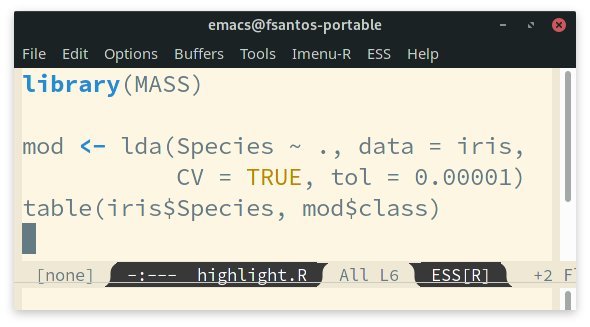
\includegraphics[width=0.5 \textwidth]{./images/highlight_default.png}
\caption{\label{fig:org07afca1}Default patterns for syntactic highlighting.}
\end{figure}

You can add more patterns to be highlighted, or remove some of them, by customizing the variable \texttt{ess-R-font-lock-keywords}.

For instance, if you also want the numbers and the function calls to be highlighted:

\begin{minted}[]{common-lisp}
;; Font lock keywords for syntactic highlighting:
(setq ess-R-font-lock-keywords
      '((ess-R-fl-keyword:keywords . t)
	(ess-R-fl-keyword:constants . t)
	(ess-R-fl-keyword:modifiers . t)
	(ess-R-fl-keyword:fun-defs . t)
	(ess-R-fl-keyword:assign-ops . t)
	(ess-R-fl-keyword:%op% . t)
	(ess-fl-keyword:fun-calls . t)
	(ess-fl-keyword:numbers . t)
	(ess-fl-keyword:operators)
	(ess-fl-keyword:delimiters)
	(ess-fl-keyword:=)
	(ess-R-fl-keyword:F&T . t))))
\end{minted}

The same code is now highlighted differently, and maybe somewhat more clearly:

\begin{figure}[htbp]
\centering
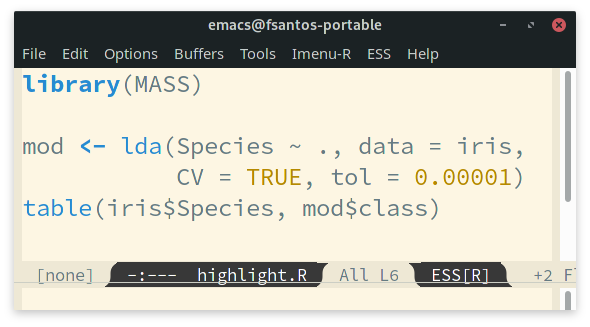
\includegraphics[width=0.55 \textwidth]{./images/highlight_custom.png}
\caption{\label{fig:org8ffbd39}More custom patterns for syntactic highlighting.}
\end{figure}

\subsection{Parenthesis matching}
\label{sec:org209103b}
\subsubsection{Seeing matching parentheses}
\label{sec:orgf46544f}
Directly taken from the ESS manual (\url{http://ess.r-project.org/Manual/ess.html\#Parens}):

\begin{quote}
``Emacs has facilities for highlighting the parenthesis matching the parenthesis at point. This feature is very useful when trying to examine which parentheses match each other. This highlighting also indicates when parentheses are not matching.''
\end{quote}

To activate parenthesis matching in ESS[R] (source) buffers, add this to your init file:

\begin{minted}[]{common-lisp}
;; Activate global mode for parenthesis matching:
(show-paren-mode)
\end{minted}

\subsubsection{Navigating through matching parentheses}
\label{sec:org5af8b38}
Here are some convenient tricks for navigating through parenthetical groups (this can be useful when dealing with large paren groups, e.g. when developing a shiny UI):

\begin{table}[htbp]
\centering
\begin{tabular}{ll}
\hline
Shortcut & \texttt{Elisp function} (Docstring)\\
\hline
\texttt{C-M-p} & \texttt{backward-list} (Move backward across one balanced paren group)\\
\texttt{C-M-n} & \texttt{forward-list} (Move forward across one balanced paren group)\\
\texttt{C-M-SPC} & \texttt{mark-sexp} (Set mark at the end of the paren group)\\
\texttt{C-M-k} & \texttt{kill-sexp} (Kill from point to end of paren group)\\
\hline
\end{tabular}
\caption{Some useful shortcuts for dealing with parenthetical groups.}

\end{table}

For instance, when the point is over a closing parenthesis, \texttt{C-M-p} brings you to the matching opening parenthesis. Then, \texttt{C-M-k} kills to whole paren group.

\subsection{Syntax checker}
\label{sec:orgfcb3839}
\subsubsection{Syntax checking: \texttt{Flycheck} vs. \texttt{Flymake}}
\label{sec:org0afd253}
ESS has facilities for on-the-fly syntax checking. Instead of using \texttt{Flymake}, which is the default choice, using \href{https://www.flycheck.org/en/latest/}{\texttt{Flycheck}} appears to be a better and more stable option. The \texttt{Flycheck} documentation allows for a comparison between those two packages:
\url{https://www.flycheck.org/en/latest/user/flycheck-versus-flymake.html}

To switch from \texttt{Flymake} to \texttt{Flycheck}, you can add the following in your init file:

\begin{minted}[]{common-lisp}
;; Remove Flymake support:
(setq ess-use-flymake nil)
;; Replace it (globally) by Flycheck:
(use-package flycheck
  :ensure t
  :init
  (global-flycheck-mode t))
\end{minted}

\subsubsection{On-the-fly syntax checking with \texttt{Flycheck}}
\label{sec:orgdd1b25c}
Using \texttt{Flycheck} with ESS first requires you to install the R package \texttt{lintr}:

\begin{minted}[]{r}
## Install stable CRAN version:
install.packages("lintr", dep = TRUE)
## OR
## Install latest Github devel version:
devtools::install_github("jimhester/lintr")
\end{minted}

(\href{https://emacs.stackexchange.com/questions/53018/flycheck-r-lintr-doesnt-find-anything}{Some users reported} that you might also have to create manually a folder \texttt{\textasciitilde{}/.R/lintr\_cache} on your computer, if it was not created after the previous step.)

\texttt{lintr} is an R package that offers facilities for static code analysis. It integrates with the main IDEs and text editors (Emacs, Rstudio, vim, etc.). In particular, it has native support for ESS + \texttt{Flycheck}.

Once both \texttt{Flycheck} and \texttt{lintr} are installed, your R code is analyzed ``on-the-fly'' while your are typing. Several checks are performed, including:
\begin{itemize}
\item R code style: correct use of \texttt{snake\_case}, convenient spacing around all operators, etc.
\item undeclared variables in function body
\item bad use of \texttt{=} for variable assignment
\item unmatched parentheses
\end{itemize}

The following screenshot (Fig. \ref{fig:org807d145}) gives some examples of such checks. To display all syntax error in a dedicated buffer, use \texttt{M-x flycheck-list-errors} (bound to \texttt{C-c ! l} by default).

\begin{figure}[htbp]
\centering
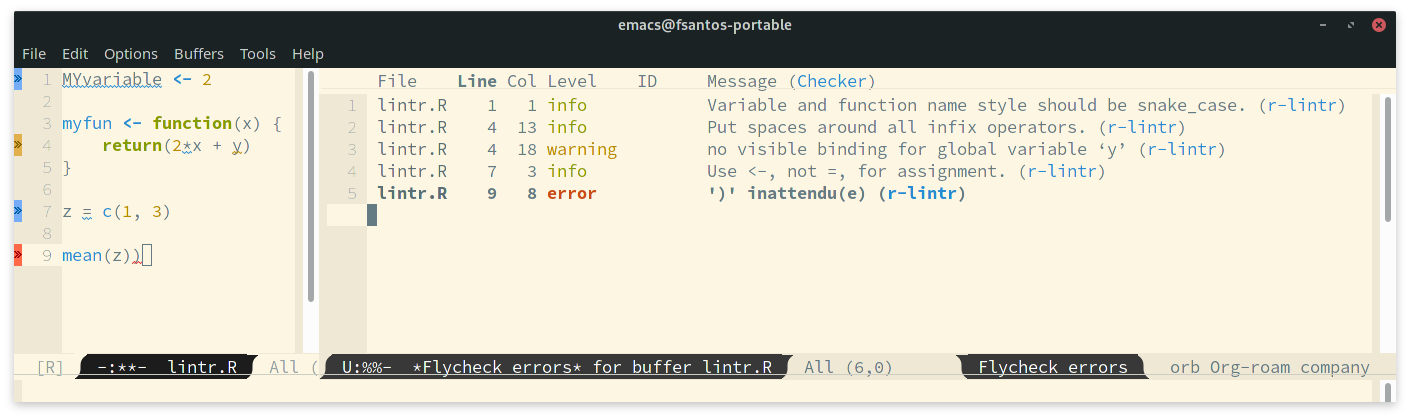
\includegraphics[width=\textwidth]{./images/lintr.png}
\caption{\label{fig:org807d145}An example of syntax errors detected by \texttt{lintr} and displayed in a dedicated \texttt{Flycheck} buffer.}
\end{figure}

\subsection{Some more steps towards an R IDE}
\label{sec:orge13061a}
\subsubsection{Rdired buffer}
\label{sec:org1063cf5}
\href{http://ess.r-project.org/Manual/ess.html\#Rdired}{From the ESS manual:}

\begin{quote}
``Ess-rdired provides a dired-like buffer for viewing, editing and plotting objects in your current R session. If you are used to using the dired (directory editor) facility in Emacs, this mode gives you similar functionality for R objects.''
\end{quote}

All the R objects of the current R sessions are thus listed in the Rdired buffer, and it is possible to interact with them easily. For instance, type \texttt{p} for plotting an object, \texttt{d} for deleting it, etc.

The screenshot in Figure \ref{fig:org3f31437} shows the contents of an Rdired buffer for the R session associated to a small piece of code.

\begin{figure}[htbp]
\centering
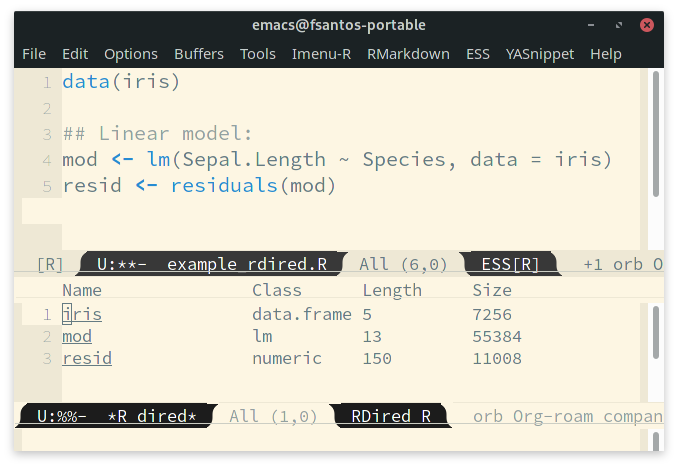
\includegraphics[width=0.75 \textwidth]{./images/rdired.png}
\caption{\label{fig:org3f31437}An example of Rdired buffer (bottom window).}
\end{figure}

Rdired buffers can be triggered manually with \texttt{M-x ess-rdired}, which might not be really convenient in practice. With the following piece of Emacs Lisp code, you will be able to use \texttt{F9} for both opening and closing the Rdired buffer, so that you can consult and display it only when necessary:

\begin{minted}[]{common-lisp}
;; Open Rdired buffer with F9:
(add-hook 'ess-r-mode-hook
	  '(lambda ()
	     (local-set-key (kbd "<f9>") #'ess-rdired)))
;; Close Rdired buffer with F9 as well:
(add-hook 'ess-rdired-mode-hook
	  '(lambda ()
	     (local-set-key (kbd "<f9>") #'kill-buffer-and-window)))
\end{minted}

\subsubsection{Window management}
\label{sec:org8b2a083}
Users coming from other R IDEs may be used to a given window (or \emph{pane}) configuration, e.g.:
\begin{itemize}
\item R source code window at the top left
\item R console (i.e., inferior R process) at the top right
\item Rdired environment window at the bottom left
\item R help window at the bottom right
\end{itemize}

This is only an arbitrary example, but quite a reasonable one. You will find in Figure \ref{fig:org856f1d7} a screenshot of such a window configuration. The corresponding Emacs Lisp code to add in your init file follows.

\begin{figure}[htbp]
\centering
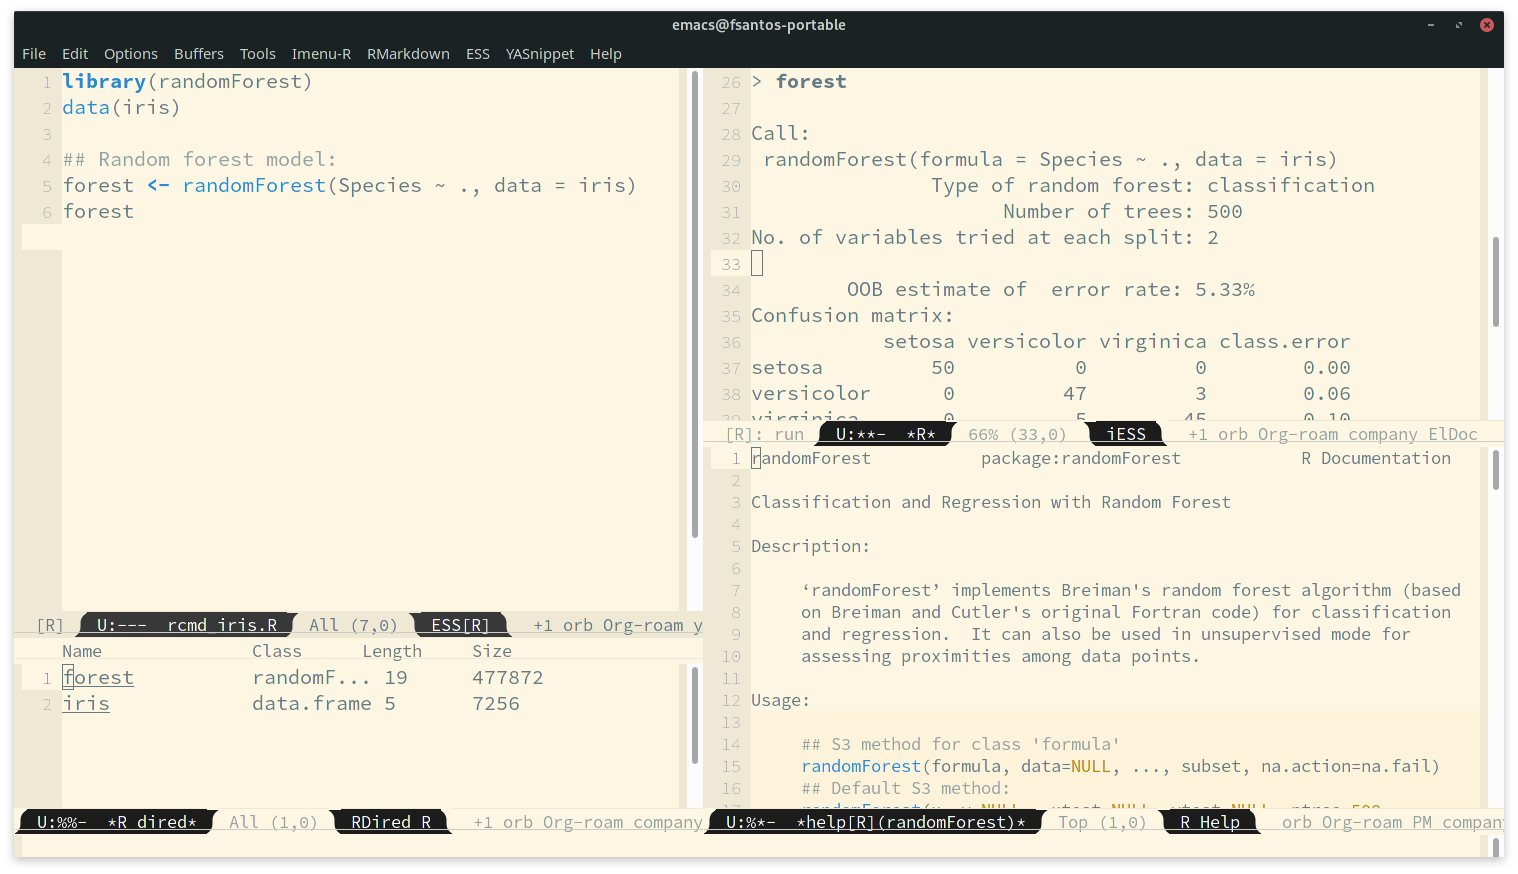
\includegraphics[width=\textwidth]{./images/window_config.png}
\caption{\label{fig:org856f1d7}An example of window configuration: ESS as an R IDE.}
\end{figure}


\begin{minted}[]{common-lisp}
;; An example of window configuration:
(setq display-buffer-alist
      '(("*R Dired"
	 (display-buffer-reuse-window display-buffer-at-bottom)
	 (window-width . 0.5)
	 (window-height . 0.25)
	 (reusable-frames . nil))
	("*R"
	 (display-buffer-reuse-window display-buffer-in-side-window)
	 (side . right)
	 (slot . -1)
	 (window-width . 0.5)
	 (reusable-frames . nil))
	("*Help"
	 (display-buffer-reuse-window display-buffer-in-side-window)
	 (side . right)
	 (slot . 1)
	 (window-width . 0.5)
	 (reusable-frames . nil))))
\end{minted}

\pagebreak

\section{Some useful Emacs packages}
\label{sec:org766105b}
\subsection{Completion with company}
\label{sec:orgda72aa3}
As mentioned \href{https://ess.r-project.org/Manual/ess.html\#Completion}{in the ESS manual}, there are several completion frameworks for writing R code with ESS. The Emacs package \href{https://company-mode.github.io/}{\texttt{company}} is an elegant solution, which also supports many other programming languages. Here is a minimal piece of Elisp code to add in your init file to install and load \texttt{company}:

\begin{minted}[]{common-lisp}
(use-package company
  :ensure t
  :config
  ;; Turn on company-mode globally:
  (add-hook 'after-init-hook 'global-company-mode)
  ;; Only activate company in R scripts, not in R console:
  (setq ess-use-company 'script-only))
\end{minted}

\begin{figure}[htbp]
\centering
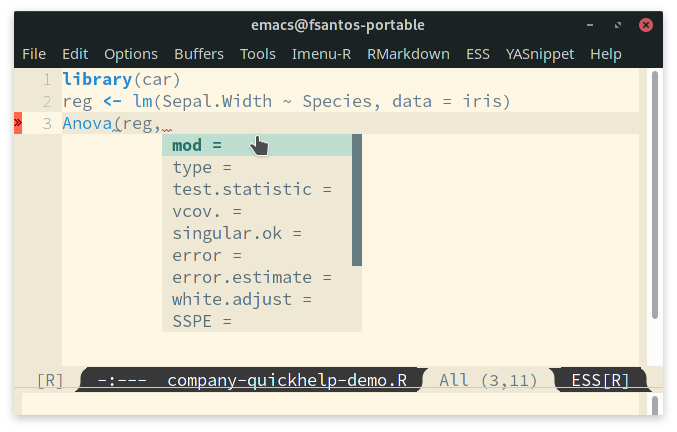
\includegraphics[width=0.64 \textwidth]{./images/company.png}
\caption{\label{fig:org6d10549}An example of code completion with \texttt{company}: various candidates are proposed for the arguments of the function \texttt{car::Anova()}.}
\end{figure}

\texttt{company} offers completion candidates in various contexts: function name, argument name within a function call (as in Fig. \ref{fig:org6d10549}), object name. It may seem preferable to adopt a non-intrusive workflow. For functions or objects names, completion starts automatically after you type a few letters. For arguments names within a function call, it is suggested that you trigger manually the completion only when you need it. This can be done with \texttt{M-x company-complete}, or more conveniently, by binding this function to a convenient shortcut. For example, to bind it to \texttt{F12}, add the following to your init file:

\begin{minted}[]{common-lisp}
;; Use F12 to trigger manually completion on R function args:
(add-hook 'ess-r-mode-hook
	  '(lambda ()
	     (local-set-key (kbd "<f12>") #'company-R-args)))
\end{minted}

\pagebreak

Of course, further customization of \texttt{company} can be done in your init file. For instance:

\begin{minted}[]{common-lisp}
;; More customization options for company:
(setq company-selection-wrap-around t
      ;; Align annotations to the right tooltip border:
      company-tooltip-align-annotations t
      ;; Idle delay in seconds until completion starts automatically:
      company-idle-delay 0.45
      ;; Completion will start after typing two letters:
      company-minimum-prefix-length 2
      ;; Maximum number of candidates in the tooltip:
      company-tooltip-limit 10)
\end{minted}

\subsection{Documentation popups with company-quickhelp}
\label{sec:org1dcae15}
\href{https://github.com/company-mode/company-quickhelp}{\texttt{company-quickhelp}} allows for documentation popups, e.g. to further describe function arguments.

\begin{figure}[htbp]
\centering
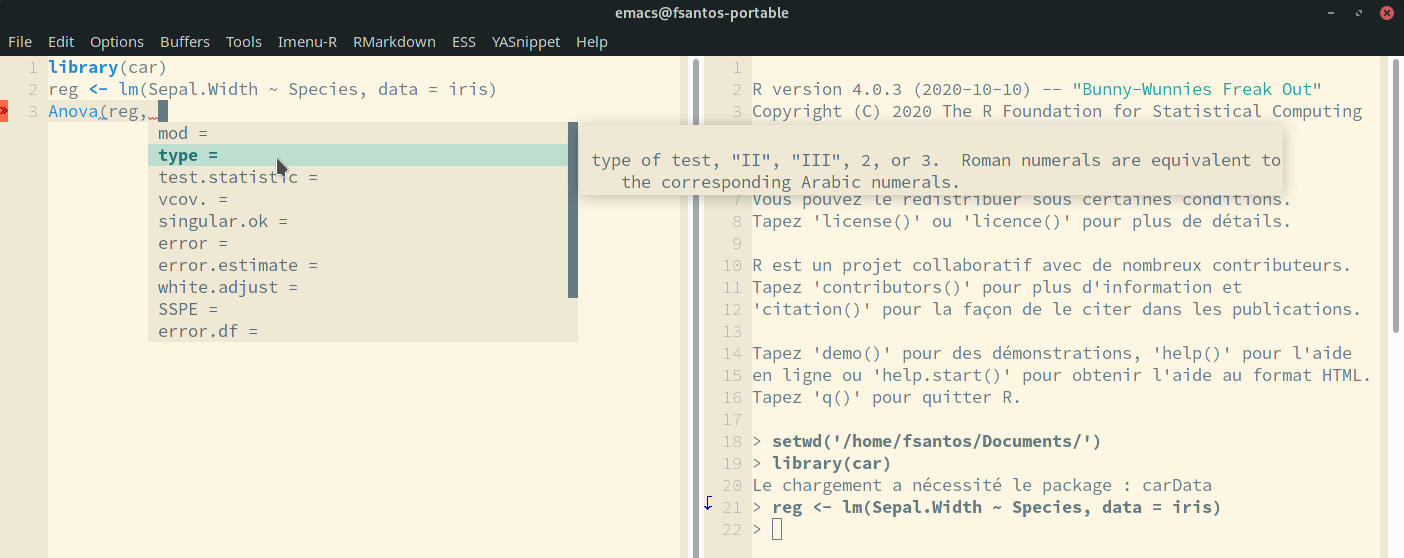
\includegraphics[width=\textwidth]{./images/company-quickhelp.png}
\caption{Documentation popups with \texttt{company-quickhelp}.}
\end{figure}

The minimal elisp code to add to your init file is straightforward:

\begin{minted}[]{common-lisp}
(use-package company-quickhelp
  :ensure t
  :config
  ;; Load company-quickhelp globally:
  (company-quickhelp-mode)
  ;; Time before display of documentation popup:
  (setq company-quickhelp-delay 0.3))
\end{minted}

By default, the documentation popup is shown automatically. You can adjust the time before the popup shows up by customizing the variable \texttt{company-quickhelp-delay}.

\subsection{Code snippets with yasnippet}
\label{sec:org20cd890}
\subsubsection{Key features}
\label{sec:org7ed9a17}
\href{https://github.com/joaotavora/yasnippet}{\texttt{yasnippet}} is an Emacs package allowing for the expansion of whole pieces of code you often use (\emph{snippets}) from one given abbreviation. 

\begin{itemize}
\item All code snippets are stored as plain-text files in one given directory, so that they are easy to share with other people, and can be easily version controlled.
\item As a corollary, it is also easy to retrieve and use large collection of snippets already available online. For instance, Andrea Crotti maintains a great collection available at \url{https://github.com/AndreaCrotti/yasnippet-snippets}.
\item Although we only demonstrate its use within ESS and R here, note that \texttt{yasnippet} is not an R-specific solution, and that you can use it for any other programming language.
\end{itemize}

\subsubsection{Setting up \texttt{yasnippet}}
\label{sec:orgd80c09f}
To set up \texttt{yasnippet}, proceed through the following steps:

\begin{enumerate}
\item Create a directory \texttt{snippets/} at some convenient location, and add a subfolder \texttt{ess-r-mode/} in this directory.
\item Add the minimal following code in your init file:
\begin{minted}[]{common-lisp}
(use-package yasnippet
  :ensure t
  :config
  ;; Indicate the directory containing your snippets:
  (setq yas-snippet-dirs '("path/to/your/snippets"))
  ;; Load your snippets on startup:
  (yas-reload-all)
  ;; Turn on yasnippet (minor) mode when editing R files:
  (add-hook 'ess-r-mode-hook #'yas-minor-mode))
\end{minted}
\item You can now fill your \texttt{snippets/ess-r-mode/} directory with your own snippets. For instance, create a file \texttt{function} (without any extension) in this directory, with the following contents:
\begin{verbatim}
#name : function
#key : fun
# --
${1:name} <- function(${2:args}) {
    ${3:body}
}
\end{verbatim}
Each snippet has a unique \texttt{name}, and can be triggered by typing a given \texttt{key} (followed by \texttt{TAB}). As we will see later on, the present snippet allows for the expansion of a template for defining new R functions more easily. The \texttt{yasnippet} manual gives more details about the expected syntax to define your own code snippets: \url{http://joaotavora.github.io/yasnippet/}.

\item Now your \texttt{snippets} directory should look like:
\begin{verbatim}
└── snippets
    └── ess-r-mode
        └── function
\end{verbatim}

Feel free to add or retrieve (a lot!) more snippets, i.e. to add more template files within the \texttt{ess-r-mode} sub-directory.
\end{enumerate}

\subsubsection{Using \texttt{yasnippet} in an ESS[R] buffer}
\label{sec:orgf1f574d}
While you are editing an R source file with ESS, each snippet can be triggered by typing its \texttt{key} and then pressing \texttt{TAB}. You can then navigate through the placeholders of the expanded template by pressing \texttt{TAB} again.

For instance, with our previously defined snippet, typing \texttt{fun} followed by \texttt{TAB} will expand the full \texttt{function} template; you will then be able to specify easily a value for each of the three placeholders (the function's \texttt{name}, its \texttt{args} and \texttt{body}).

Note that \texttt{yasnippet} has a short video tutorial, available at \url{https://www.youtube.com/watch?v=ZCGmZK4V7Sg}.
\end{document}